\documentclass[10pt,a4paper]{article}
\usepackage{fontspec}
\setmainfont{Times New Roman}[
  Path=/System/Library/Fonts/Supplemental/,
  UprightFont=Times New Roman.ttf,
  BoldFont=Times New Roman Bold.ttf,
  ItalicFont=Times New Roman Italic.ttf,
  BoldItalicFont=Times New Roman Bold Italic.ttf
]
\usepackage[margin=1.75cm]{geometry}
\usepackage{amsmath,amssymb,booktabs,graphicx,microtype,url,array,float}
\usepackage[hidelinks]{hyperref}
\renewcommand{\abstractname}{Tóm tắt}
\renewcommand{\tablename}{Bảng}
\renewcommand{\figurename}{Hình}
\renewcommand{\refname}{Tài liệu tham khảo}
\title{PHÂN LOẠI CIFAR-10 BẰNG DEEP LEARNING VÀ VISION TRANSFORMER}
\author{Hồ Võ Hoàng Duy - 25C01002}
\date{Ngày 3 tháng 10 năm 2026}

\begin{document}
\maketitle

\begin{abstract}
Báo cáo nghiên cứu phân loại ảnh CIFAR-10 bằng các mô hình học sâu AlexNet,
VGG11, ResNet18 và Vision Transformer (ViT tiny). Các kiến trúc được điều chỉnh
cho ảnh $32\times32$, cài đặt bằng các lớp cơ bản của PyTorch và huấn luyện từ
trọng số ngẫu nhiên, không sử dụng pretrained. Thực nghiệm dùng 45.000 ảnh huấn
luyện, 5.000 ảnh kiểm định và 10.000 ảnh kiểm tra; mỗi mạng được huấn luyện 200
epoch và chọn checkpoint theo accuracy kiểm định. Sáu cấu hình Pixel, HOG và
SIFT phẳng kết hợp SVM hoặc Random Forest được giữ làm mốc so sánh.
AlexNet đạt accuracy 83,87\% và macro-F1 0,8381, cao nhất trong các cấu hình
đã chạy; ViT tiny đạt 68,21\%. Báo cáo phân tích hiệu quả học biểu diễn,
chi phí huấn luyện và giới hạn tổng quát hóa của các mô hình.
\end{abstract}

\section{Giới thiệu}
Phân loại ảnh yêu cầu mô hình nhận biết đối tượng dù góc nhìn, màu sắc và nền
thay đổi. CIFAR-10 gồm 60.000 ảnh màu $32\times32$ thuộc 10 lớp, là bộ dữ liệu
phù hợp để khảo sát bài toán này ở độ phân giải thấp \cite{krizhevsky2009cifar}.
Thay vì cố định cách trích xuất đặc trưng trước khi học bộ phân lớp, học sâu
đồng thời tối ưu biểu diễn ảnh và quyết định phân lớp từ dữ liệu.

Báo cáo tập trung vào hai hướng: mạng tích chập (CNN) và Vision Transformer.
AlexNet dùng chuỗi tích chập, ReLU và pooling; VGG tổ chức các tích chập nhỏ theo
chiều sâu; ResNet bổ sung kết nối tắt để học phần dư
\cite{krizhevsky2012alexnet,simonyan2015vgg,he2016resnet}.
ViT biểu diễn ảnh bằng một chuỗi patch và dùng self-attention để trao đổi thông
tin giữa các vùng ảnh \cite{dosovitskiy2021vit}.

Mục tiêu là cài đặt các biến thể AlexNet, VGG11, ResNet18 và ViT tiny cho
CIFAR-10, huấn luyện từ đầu và đánh giá accuracy cùng macro-F1 trên tập kiểm tra
chính thức. Các kết quả truyền thống được giữ lại để đo mức cải thiện so với
biểu diễn pixel thô hoặc đặc trưng thiết kế thủ công. Phần phương pháp tập trung
vào học sâu; các baseline chỉ được mô tả ngắn gọn để giải thích phép so sánh.

\section{Dữ liệu và tiền xử lý}
CIFAR-10 cung cấp 50.000 ảnh train và 10.000 ảnh test chính thức
\cite{krizhevsky2009cifar}. Từ tập train, phép chia phân tầng với seed 42 giữ
45.000 ảnh để huấn luyện và 5.000 ảnh để kiểm định. Test giữ nguyên 10.000 ảnh
và được đánh giá sau khi chọn checkpoint của mỗi mạng.

\begin{table}[H]
\centering
\caption{Phân chia dữ liệu cho các thí nghiệm.}
\label{tab:split}
\begin{tabular}{lrrl}
\toprule
Tập & Số ảnh & Số ảnh/lớp & Vai trò \\
\midrule
Huấn luyện & 45.000 & 4.500 & Học thống kê chuẩn hóa và trọng số \\
Kiểm định & 5.000 & 500 & Chọn checkpoint học sâu \\
Kiểm tra & 10.000 & 1.000 & Đánh giá cuối \\
\bottomrule
\end{tabular}
\end{table}

\textbf{Đầu vào học sâu.} Ảnh giữ nguyên ba kênh RGB và kích thước
$32\times32$. Giá trị pixel được chuyển về $[0,1]$, rồi chuẩn hóa theo từng kênh:
\begin{equation}
 \hat{I}_{c,h,w}=\frac{I_{c,h,w}/255-\mu_c^{\mathrm{train}}}
 {\max(\sigma_c^{\mathrm{train}},10^{-6})}.
\end{equation}
Trung bình và độ lệch chuẩn được tính trên tập train, sau đó giữ cố định cho
validation và test. Lần chạy này không dùng tăng cường dữ liệu như lật ảnh,
cắt ngẫu nhiên hoặc biến đổi màu.

\textbf{Đầu vào baseline.} Pixel thô được trải phẳng thành 3.072 chiều.
HOG và SIFT dùng ảnh xám $I=0.299R+0.587G+0.114B$; vector đặc trưng được chuẩn
hóa theo từng chiều bằng thống kê của train. Hai nhánh dùng cách chuẩn hóa phù
hợp với loại đầu vào, không dùng thống kê test để học tham số.

\subsection{Tổng quan pipeline}
\begin{figure}[H]
\centering
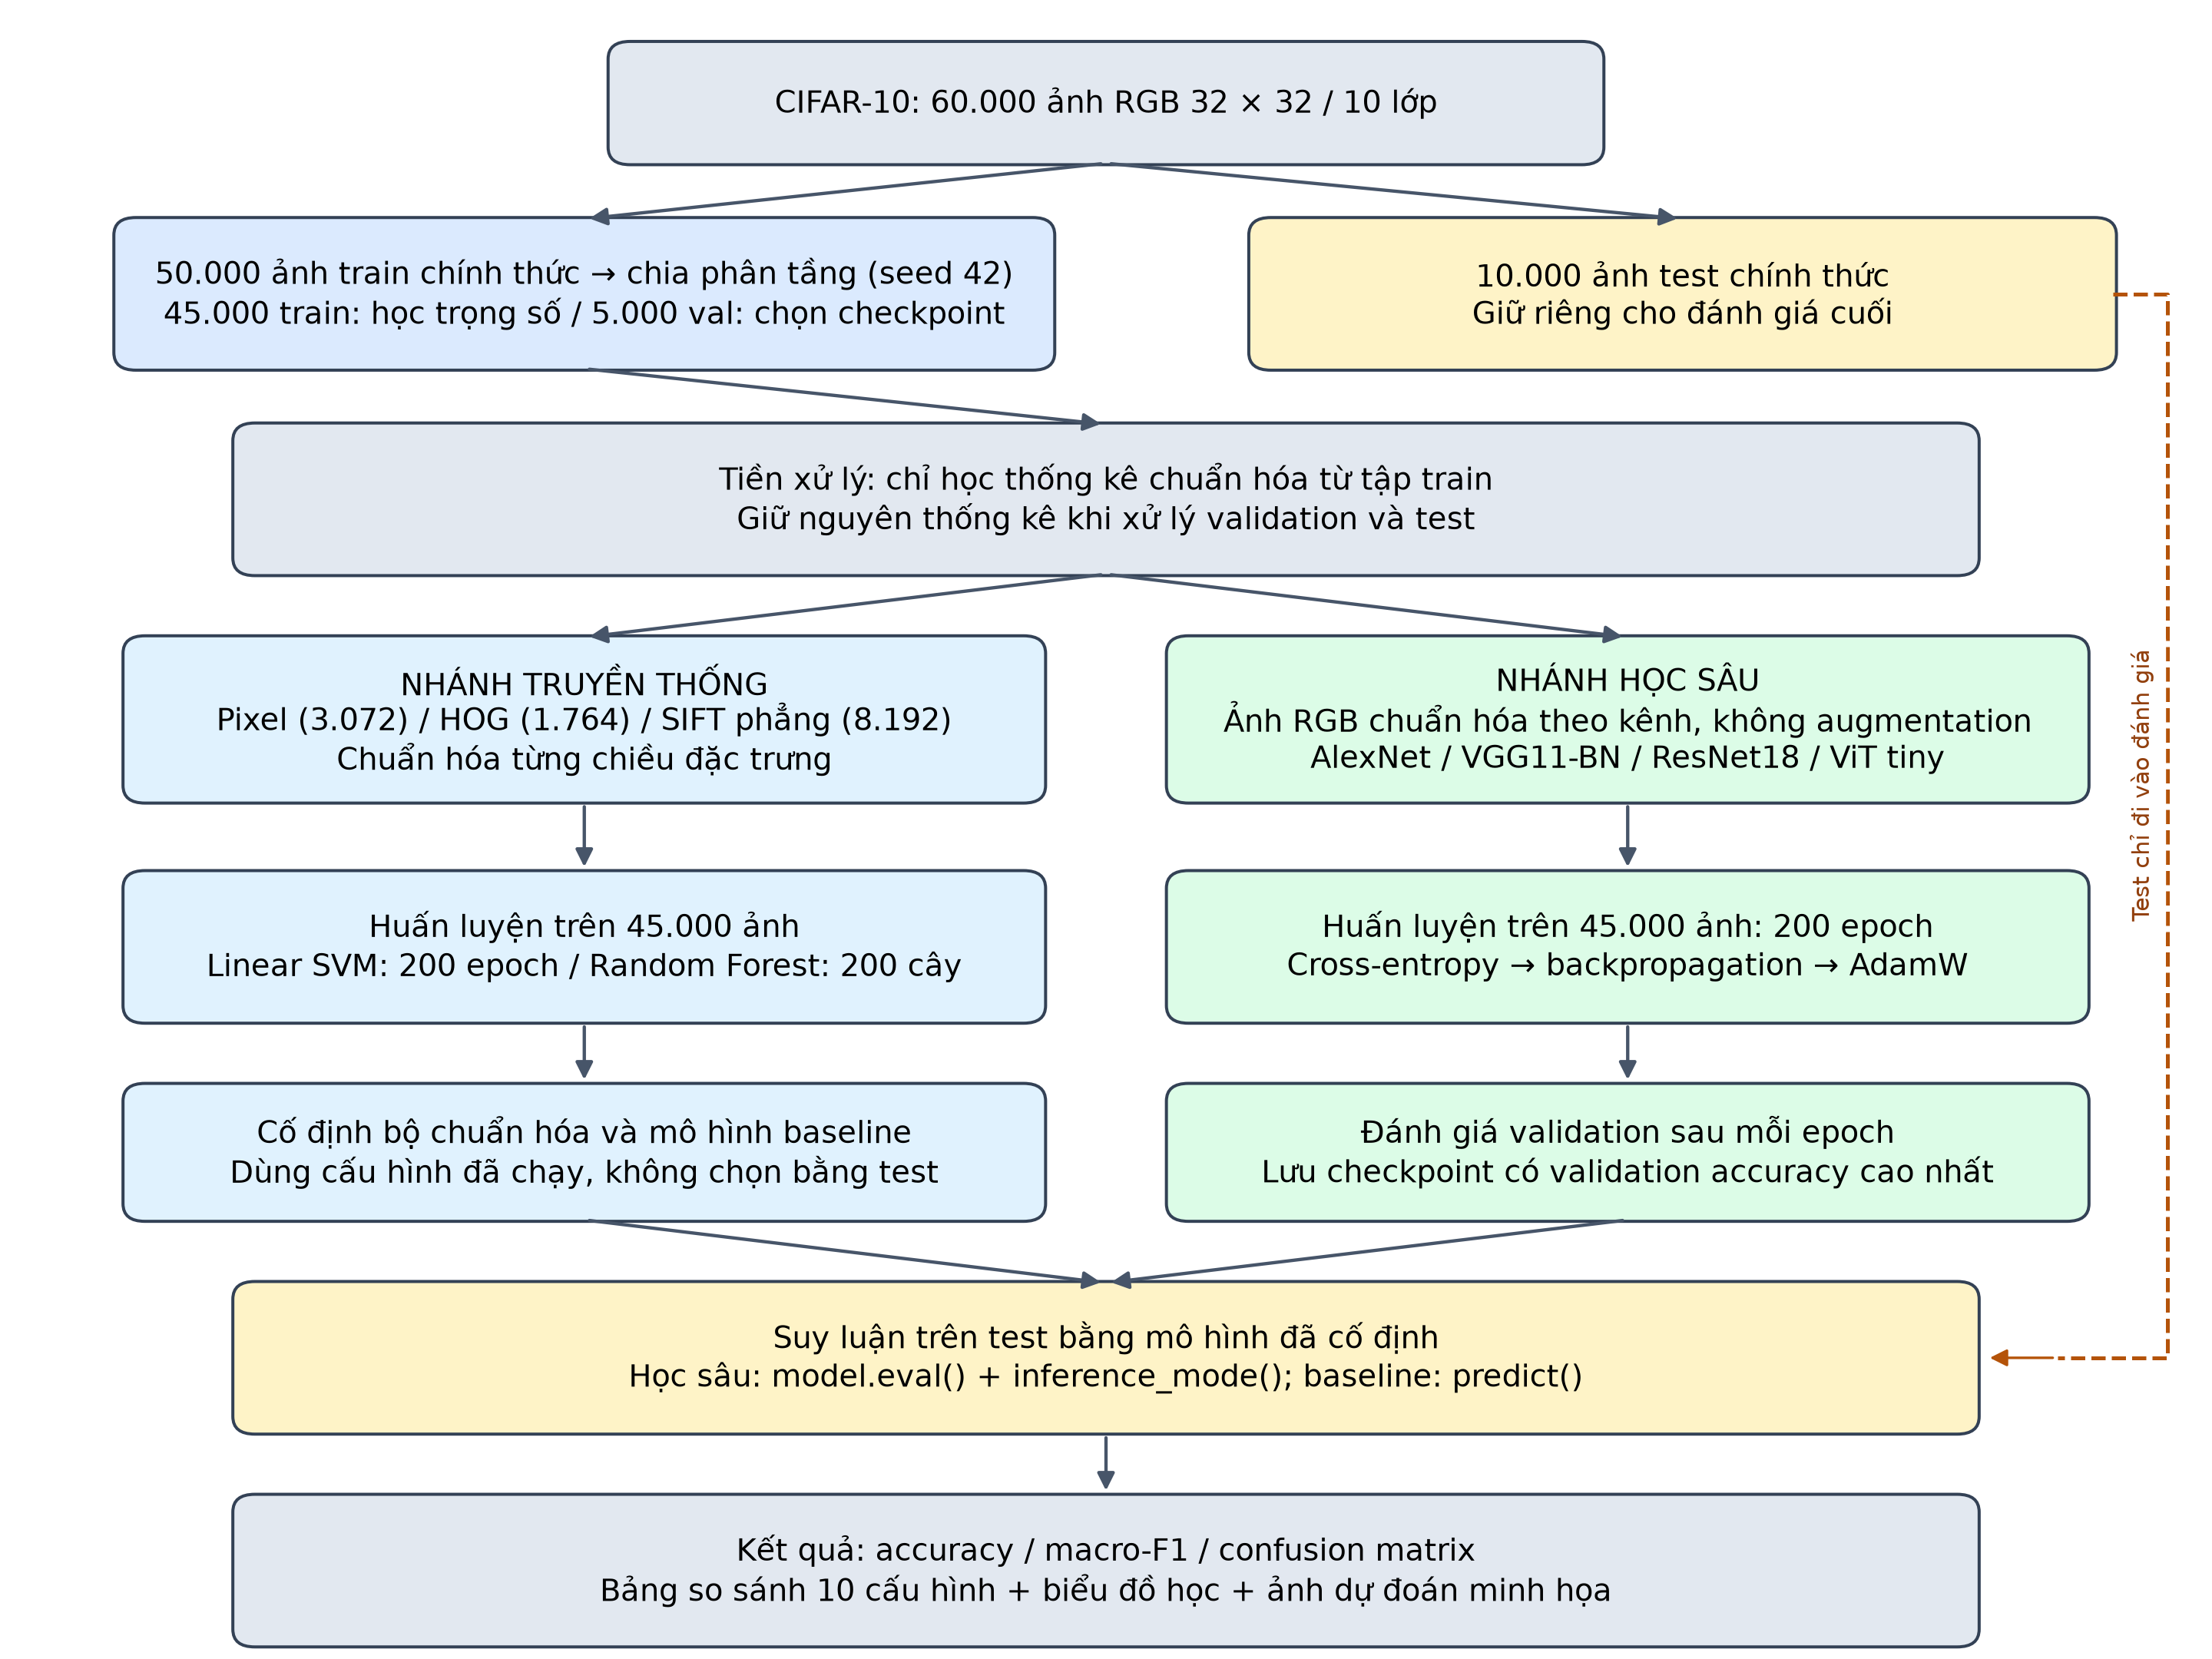
\includegraphics[width=0.96\linewidth]{assets/figures/pipeline_overview.png}
\caption{Pipeline tổng quan: hai nhánh dùng cùng cỡ dữ liệu, chỉ học thống kê chuẩn hóa từ train; validation chọn checkpoint học sâu và test chỉ đi vào đánh giá cuối.}
\label{fig:pipeline}
\end{figure}
Hình~\ref{fig:pipeline} phân biệt bước học tham số với bước đánh giá.
Nhánh truyền thống dùng đặc trưng cố định rồi học SVM hoặc Random Forest;
nhánh học sâu tối ưu đồng thời biểu diễn và bộ phân lớp. Sau khi cố định mô
hình và thống kê chuẩn hóa, test được xử lý và suy luận để tạo các chỉ số
so sánh. Ảnh dự đoán minh họa được lấy từ checkpoint đã chọn, không dùng để
chọn lại trọng số hoặc điều chỉnh siêu tham số.

\section{Phương pháp học sâu}
Các kiến trúc trong phần này được mô tả theo cài đặt tại
\path{deep_models/models.py}. Kích thước tensor được ghi theo thứ tự
$C\times H\times W$ cho CNN; $T\times D$ cho ViT; bỏ qua chiều batch $B$.
Đây là các biến thể cho CIFAR-10, với trọng số được học từ đầu.

\subsection{Nguyên lý chung: học biểu diễn và tối ưu đầu-cuối}
\textbf{Tích chập.} Một lớp convolution tạo mỗi kênh đầu ra bằng cách kết hợp
các vùng lân cận trên tất cả kênh đầu vào:
\begin{equation}
 a_{o,h,w}=b_o+\sum_{c=1}^{C_{in}}\sum_{u,v}
 W_{o,c,u,v}\,x_{c,sh+u-p,sw+v-p}.
\end{equation}
Kernel $W$ được dùng lại ở nhiều vị trí; $s$ là stride, $p$ là padding.
Với kích thước đầu vào $H$, kernel $k$ và dilation 1, kích thước đầu ra là
$H_{out}=\lfloor(H+2p-k)/s\rfloor+1$.
Ví dụ, kernel $3\times3$, padding 1 và stride 1 giữ nguyên kích thước;
stride 2 giảm khoảng một nửa. Việc chia sẻ trọng số giúp cùng một mẫu cạnh
được phát hiện ở nhiều vị trí mà không học một bộ trọng số riêng cho từng pixel.

\textbf{Phi tuyến và gộp thông tin.} ReLU, $\max(0,a)$, làm mạng có khả năng
biểu diễn quan hệ phi tuyến. Nếu chỉ ghép các lớp tuyến tính, toàn mạng vẫn là
một phép biến đổi tuyến tính, dù có nhiều lớp. Max-pooling $2\times2$, stride 2
chọn đáp ứng lớn nhất trong mỗi vùng, giảm kích thước và độ nhạy với dịch chuyển
nhỏ; nó cũng có thể làm mất chi tiết trên ảnh nhỏ. Global average pooling lấy
trung bình trên toàn bộ vùng không gian của từng kênh. Qua nhiều lớp, vùng ảnh
ảnh hưởng đến một đặc trưng (receptive field) mở rộng; biểu diễn có thể kết hợp
mẫu cục bộ thành cấu trúc lớn hơn phục vụ phân lớp.

\textbf{Học biểu diễn.} Mạng phân loại được viết thành
$z=g_\theta(f_\phi(I))$, trong đó $f_\phi$ là bộ trích xuất đặc trưng học được,
$g_\theta$ là bộ phân lớp và $z$ có 10 logit. Với đặc trưng thủ công $h(I)$,
chỉ bộ phân lớp được học; với học sâu, cả $\phi$ và $\theta$ nhận gradient từ
cùng mục tiêu. Chẳng hạn, nếu một mẫu màu hoặc đường biên giúp phân biệt
\emph{ship} với \emph{airplane}, trọng số phía trước có thể được điều chỉnh để
làm nổi bật mẫu đó. Đây là khả năng của mô hình, không phải khẳng định rằng
mọi bộ lọc trong lần chạy này đã được giải thích về mặt ngữ nghĩa.

\textbf{Hàm mất mát và quy trình cập nhật.} Với logit $z_{ik}$:
\begin{equation}
 p_{ik}=\frac{\exp(z_{ik})}{\sum_{j=1}^{10}\exp(z_{ij})},\qquad
 \mathcal{L}_{CE}=-\frac{1}{B}\sum_{i=1}^{B}\log p_{i,y_i}.
\end{equation}
Mỗi mini-batch được chuẩn hóa, đưa qua mạng, tính cross-entropy, lan truyền
ngược và cập nhật bằng AdamW. Đạo hàm loss theo logit của một mẫu tỉ lệ với
$p_{ik}-\mathbf{1}[k=y_i]$, nên lớp sai có điểm cao nhận tín hiệu điều chỉnh
mạnh. Gradient norm được giới hạn ở 1,0 trước bước optimizer; weight decay
$10^{-4}$ giúp kiểm soát độ lớn trọng số. Các cơ chế này không bảo đảm hết
quá khớp, vì còn phụ thuộc dữ liệu, kiến trúc và thời gian huấn luyện.

\textbf{Đánh giá.} Sau mỗi epoch, mạng chuyển sang chế độ evaluation để đo
accuracy validation và lưu checkpoint tốt nhất. Khi suy luận, dropout được
vô hiệu hóa, BatchNorm dùng thống kê đã tích lũy; trọng số không cập nhật.
Nhãn cuối là $\hat y=\arg\max_k z_k$. Softmax chỉ chuyển logit thành phân bố
điểm tổng bằng 1; điểm cao không bảo đảm dự đoán đúng hay xác suất đã được hiệu chuẩn.

\subsection{AlexNet với GroupNorm}
\textbf{Ý tưởng kiến trúc.} AlexNet sử dụng tích chập, ReLU, pooling và
bộ phân lớp có dropout \cite{krizhevsky2012alexnet}. Biến thể CIFAR-10 gồm
năm convolution, với GroupNorm sau mỗi lớp. Các convolution có stride 1;
padding 2 cho kernel $5\times5$ và padding 1 cho kernel $3\times3$.
Vì vậy, chỉ các lớp pooling làm giảm kích thước không gian.

\begin{table}[H]
\centering\small
\caption{Luồng tensor của AlexNet trong thí nghiệm. Conv được theo sau bởi GroupNorm và ReLU.}
\begin{tabular}{lll}
\toprule
Bước & Thao tác & Đầu ra \\
\midrule
Đầu vào & RGB đã chuẩn hóa & $3\times32\times32$ \\
1 & Conv $5\times5$, 64 kênh; max-pool & $64\times16\times16$ \\
2 & Conv $3\times3$, 192 kênh; max-pool & $192\times8\times8$ \\
3 & Conv $3\times3$, 384 kênh & $384\times8\times8$ \\
4 & Conv $3\times3$, 256 kênh & $256\times8\times8$ \\
5 & Conv $3\times3$, 256 kênh; max-pool & $256\times4\times4$ \\
6 & Adaptive average pooling $2\times2$; flatten & $1024$ \\
7 & Dropout; Linear $1024\rightarrow512$; ReLU & $512$ \\
8 & Dropout; Linear $512\rightarrow10$ & $10$ logit \\
\bottomrule
\end{tabular}
\end{table}

\textbf{GroupNorm.} Tại mỗi mẫu, các kênh được chia thành tám nhóm. Trung bình
và phương sai được tính trên các kênh và vị trí không gian trong từng nhóm,
không trên batch \cite{wu2018groupnorm}. Nếu $\mathcal{G}$ là nhóm chứa $a_j$:
\begin{equation}
 \hat a_j=\gamma_j\frac{a_j-\mu_{\mathcal G}}
 {\sqrt{\sigma_{\mathcal G}^2+\epsilon}}+\beta_j.
\end{equation}
Với lớp 64 kênh, mỗi nhóm có tám kênh; với lớp 192 kênh, mỗi nhóm có 24 kênh.
Hệ số scale và bias được học cùng mạng. GroupNorm không cần running mean
và running variance như BatchNorm, nên cách tính thống kê không phụ thuộc số
mẫu trong mini-batch. Không thể từ đó kết luận GroupNorm là nguyên nhân duy nhất
khiến AlexNet đạt kết quả cao nhất; cần thí nghiệm thay riêng lớp chuẩn hóa.

\textbf{Bộ phân lớp và điều chuẩn.} Adaptive pooling giữ lưới $2\times2$,
cho phép vector cuối còn thông tin vị trí thô. Hai lớp tuyến tính học tổ hợp
phi tuyến của các đặc trưng tích chập. Dropout 0,5 ngẫu nhiên loại bỏ một nửa
phần tử ở vị trí dropout khi train và điều chỉnh tỉ lệ phần tử còn lại; khi
inference dùng toàn bộ phần tử. Cơ chế này hạn chế việc bộ phân lớp phụ thuộc
quá mạnh vào một số đặc trưng. Mạng có 2.786.890 tham số. So với AlexNet
ImageNet, ảnh đầu vào, kernel, pooling, chuẩn hóa và classifier đều đã được
điều chỉnh; vì vậy tên kiến trúc cần được đọc cùng cấu hình trên.

\subsection{VGG11-BN với số kênh giảm}
\textbf{Ý tưởng kiến trúc.} VGG dùng các convolution $3\times3$ xếp chồng
\cite{simonyan2015vgg}. Bản cài đặt dùng tám convolution, mỗi lớp có padding 1,
stride 1, theo sau bởi BatchNorm và ReLU. Hai lớp $3\times3$ liên tiếp có vùng
nhìn danh nghĩa $5\times5$ trong trường hợp stride 1, đồng thời bổ sung một
phép phi tuyến giữa chúng. Năm pooling giảm dần kích thước ảnh về $1\times1$.

\begin{table}[H]
\centering\small
\caption{Năm stage của VGG11-BN. Mỗi stage kết thúc bằng max-pooling $2\times2$.}
\begin{tabular}{lllr}
\toprule
Stage & Các convolution $3\times3$ & Đầu ra sau pooling & Số conv \\
\midrule
1 & $3\rightarrow32$ & $32\times16\times16$ & 1 \\
2 & $32\rightarrow64$ & $64\times8\times8$ & 1 \\
3 & $64\rightarrow128\rightarrow128$ & $128\times4\times4$ & 2 \\
4 & $128\rightarrow256\rightarrow256$ & $256\times2\times2$ & 2 \\
5 & $256\rightarrow256\rightarrow256$ & $256\times1\times1$ & 2 \\
\bottomrule
\end{tabular}
\end{table}

\textbf{BatchNorm.} Với mỗi kênh, BatchNorm chuẩn hóa activation bằng trung
bình và phương sai của các mẫu và vị trí không gian trong mini-batch lúc train,
rồi học scale và bias \cite{ioffe2015batchnorm}. Khi evaluation, lớp này dùng
thống kê tích lũy thay vì tính lại theo batch test. Điều này làm thao tác train
và inference khác nhau; chế độ \texttt{model.eval()} là cần thiết để suy luận
đúng. Khác với GroupNorm của AlexNet, thống kê lúc train phụ thuộc batch.

\textbf{Phân lớp và đánh đổi.} Sau stage 5, flatten tạo 256 đặc trưng, đưa
thẳng vào lớp tuyến tính $256\rightarrow10$; không dùng các fully connected lớn
của VGG nguyên bản và không có dropout trong cài đặt này. Mạng có 2.310.186
tham số, ít nhất trong bốn mạng. Cấu trúc tuần tự dễ triển khai nhưng việc giảm
$32\rightarrow16\rightarrow8\rightarrow4\rightarrow2\rightarrow1$ có thể
làm mất chi tiết ở ảnh nhỏ. Dữ liệu không xác nhận riêng tác động của pooling;
đây là một yếu tố cần kiểm tra khi giải thích chênh lệch với các mạng khác.

\subsection{ResNet18 với kết nối phần dư}
\textbf{BasicBlock.} Mỗi block chứa hai convolution $3\times3$ kèm BatchNorm;
ReLU đặt sau convolution thứ nhất và sau phép cộng nhánh tắt. Viết chi tiết:
\begin{align}
 F(x)&=\mathrm{BN}_2\bigl(\mathrm{Conv}_2(
       \mathrm{ReLU}(\mathrm{BN}_1(\mathrm{Conv}_1(x))))\bigr),\\
 y&=\mathrm{ReLU}\bigl(F(x)+S(x)\bigr).
\end{align}
Khi số kênh và kích thước không đổi, $S(x)=x$. Khi đổi kênh hoặc stride 2,
$S$ là convolution $1\times1$ với cùng stride và BatchNorm, để hai nhánh có
cùng shape trước phép cộng. Hai convolution trong nhánh $F$ không có bias
vì đã đi kèm BatchNorm.

\textbf{Vì sao học phần dư?} Thay vì học toàn bộ ánh xạ $H(x)$, nhánh biến đổi
học $F(x)=H(x)-x$ khi dùng identity shortcut \cite{he2016resnet}.
Bỏ qua ReLU để xét phép cộng, đạo hàm theo đầu vào là
$\partial(F(x)+x)/\partial x=\partial F/\partial x+I$.
Hạng $I$ tạo đường truyền trực tiếp cho gradient. ReLU sau phép cộng vẫn có
thể chặn một số thành phần; shortcut giúp tối ưu thuận lợi hơn nhưng không
bảo đảm mọi gradient luôn được giữ nguyên hoặc mạng sâu luôn tốt hơn.

\begin{table}[H]
\centering\small
\caption{Các stage của ResNet18 CIFAR; mỗi stage có hai BasicBlock.}
\begin{tabular}{llll}
\toprule
Phần & Số kênh & Stride block đầu & Đầu ra \\
\midrule
Stem: Conv $3\times3$ + BN + ReLU & 32 & 1 & $32\times32\times32$ \\
Stage 1 & 32 & 1 & $32\times32\times32$ \\
Stage 2 & 64 & 2 & $64\times16\times16$ \\
Stage 3 & 128 & 2 & $128\times8\times8$ \\
Stage 4 & 256 & 2 & $256\times4\times4$ \\
Global average pooling; linear & 256 & -- & $256\rightarrow10$ \\
\bottomrule
\end{tabular}
\end{table}

\textbf{Điều chỉnh cho ảnh nhỏ.} Stem dùng kernel $3\times3$, stride 1,
không max-pooling đầu mạng để giữ chi tiết ở độ phân giải $32\times32$.
Tám BasicBlock có tổng 16 convolution trên nhánh chính; thêm convolution stem
và lớp tuyến tính cuối tạo cấu trúc ResNet18 thông dụng (không đếm riêng
convolution projection trong cách gọi này). Base width giảm còn 32, nên mạng
có 2.797.610 tham số. Global average pooling lấy trung bình trên $4\times4$
cho mỗi kênh, giảm số tham số classifier. ResNet có đường truyền gradient
thuận lợi, nhưng mức accuracy cuối vẫn phụ thuộc cách chuẩn hóa, điều chuẩn,
lịch learning rate và khả năng tổng quát hóa trên dữ liệu đã chọn.

\subsection{Vision Transformer: ViT tiny}
\textbf{Bước 1: biến ảnh thành token.} Cài đặt dùng convolution kernel 4,
stride 4 để nhúng patch. Ảnh $3\times32\times32$ tạo lưới $8\times8$ patch;
mỗi patch có $4\times4\times3=48$ giá trị và được ánh xạ thành vector 192 chiều.
Flatten lưới và chuyển trục tạo tensor $64\times192$. Thêm class token và
embedding vị trí học được:
\begin{equation}
 Z_0=[x_{cls};\,x_p^1E;\ldots;x_p^{64}E]+E_{pos},\quad
 E\in\mathbb{R}^{48\times192},\quad E_{pos}\in\mathbb{R}^{65\times192}.
\end{equation}
Phép chiếu patch thực tế còn có bias. Class token là một vector học được,
không phải ảnh hay nhãn thật; nó thu thập thông tin cho quyết định phân lớp.
Embedding vị trí phân biệt các vị trí trong lưới, vì attention đơn thuần không
mã hóa thứ tự không gian \cite{dosovitskiy2021vit}.

\textbf{Bước 2: self-attention ba head.} Trong mỗi block, LayerNorm chuẩn hóa
192 chiều của từng token; một lớp tuyến tính tạo $Q,K,V$. Mỗi head có
$Q_h,K_h,V_h\in\mathbb{R}^{65\times64}$:
\begin{equation}
 A_h=\operatorname{softmax}_{\mathrm{hàng}}\left(
 \frac{Q_hK_h^\top}{\sqrt{64}}\right),\qquad U_h=A_hV_h.
\end{equation}
Mỗi hàng của $A_h\in\mathbb{R}^{65\times65}$ biểu diễn trọng số kết hợp các
token cho một token truy vấn. Ba $U_h$ được nối thành 192 chiều rồi chiếu
bằng lớp tuyến tính. Các head có thể học những kiểu quan hệ khác nhau, nhưng
không có ràng buộc rằng mỗi head phải tương ứng một bộ phận vật thể cụ thể.
Việc trao đổi thông tin diễn ra giữa mọi cặp token ngay trong một block,
khác với tích chập chỉ kết hợp lân cận tại từng lớp.

\textbf{Bước 3: MLP và kết nối phần dư.} Sáu block dùng cấu trúc pre-norm,
đúng theo thứ tự trong mã nguồn:
\begin{align}
 Z'_\ell&=Z_{\ell-1}+\mathrm{MSA}(\mathrm{LN}(Z_{\ell-1})),\\
 Z_\ell&=Z'_\ell+\mathrm{MLP}(\mathrm{LN}(Z'_\ell)),\\
 \mathrm{MLP}(u)&=W_2\,\mathrm{GELU}(W_1u+b_1)+b_2.
\end{align}
MLP mở rộng $192\rightarrow768$ rồi thu về $192$, xử lý từng token với cùng
trọng số; self-attention đảm nhiệm trao đổi giữa token. LayerNorm không dùng
thống kê batch hay running statistics. Shape $65\times192$ không đổi qua
sáu block; hai nhánh cộng phần dư giúp giữ thông tin đầu vào block.

\begin{table}[H]
\centering\small
\caption{Luồng tensor của ViT tiny trong cài đặt.}
\begin{tabular}{lll}
\toprule
Bước & Cấu hình & Đầu ra \\
\midrule
Patch embedding & Conv kernel 4, stride 4, 192 kênh & $192\times8\times8$ \\
Chuỗi token & Flatten lưới; thêm class token và vị trí & $65\times192$ \\
Encoder & 6 block; 3 head; MLP ratio 4 & $65\times192$ \\
Đầu phân lớp & LayerNorm; lấy class token; Linear & $192\rightarrow10$ \\
\bottomrule
\end{tabular}
\end{table}

\textbf{Bước 4: phân lớp và giới hạn.} Sau encoder, LayerNorm được áp dụng
cho biểu diễn class token trước lớp tuyến tính 10 logit. Mạng có 2.693.578
tham số, không có dropout trong các block và không dùng pretrained.
Chi phí tạo attention tăng theo $T^2$ với $T=65$; mỗi head có 4.225 trọng số
attention cho một ảnh. Patch lớn làm chuỗi ngắn hơn nhưng gom nhiều pixel vào
một token; patch nhỏ tăng số token và chi phí. Trong cấu hình này, ViT có
khả năng mô hình hóa quan hệ toàn ảnh nhưng phải học từ lượng dữ liệu tương
đối hạn chế. Cấu trúc đó không tự bảo đảm accuracy cao hơn CNN.

\subsection{Các phương pháp truyền thống làm mốc so sánh}
Pixel được trải phẳng thành 3.072 chiều, giữ thứ tự các vị trí RGB nhưng không
có cơ chế tích chập hay chia sẻ trọng số theo không gian. HOG chia ảnh xám thành
cell $4\times4$, tính histogram 9 hướng gradient, chuẩn hóa trên block
$2\times2$ chồng lấn và nối thành 1.764 chiều \cite{dalal2005hog}.
HOG giữ bố cục gradient ở lưới cố định, nhưng không giữ trực tiếp màu RGB.

SIFT phẳng tìm keypoint trong một octave, gán hướng và mô tả mỗi điểm bằng
128 giá trị; tối đa 64 descriptor được xếp theo độ mạnh, nối và đệm số 0,
thành 8.192 chiều \cite{lowe2004sift}. Cài đặt này rút gọn SIFT và không dùng
Bag of Visual Words. Khi keypoint thay đổi thứ tự giữa các ảnh, một chiều
trong vector không còn chắc chắn mang cùng ý nghĩa; việc phóng ảnh nhỏ lên
cũng không tạo thêm chi tiết thị giác thực sự.

SVM tuyến tính học các điểm số $s_k=w_k^\top x+b_k$ bằng hinge loss đa lớp
và điều chuẩn L2 \cite{cortes1995svm}. Dù có nhiều chiều, ranh giới trong
không gian đặc trưng vẫn tuyến tính. Random Forest dùng nhiều cây học từ mẫu
bootstrap, chọn ngẫu nhiên đặc trưng khi chia nút và bỏ phiếu nhãn
\cite{breiman2001random}. Các cây tạo ranh giới phi tuyến nhưng không có
cơ chế chuyên biệt để ghép mẫu cục bộ thành biểu diễn ảnh nhiều tầng.
Sáu kết quả của hai bộ phân lớp trên ba loại đầu vào được giữ nguyên trong
bảng so sánh; chúng là baseline cho cấu hình học sâu đã khảo sát.


\section{Thiết lập thí nghiệm}
Bốn mạng được định nghĩa bằng các lớp cơ bản của PyTorch, khởi tạo ngẫu nhiên
và huấn luyện độc lập trên MPS; không dùng model zoo hay pretrained weights.
Cùng seed 42, số mẫu train/validation/test là 45.000/5.000/10.000.
Mỗi mạng chạy 200 epoch với AdamW, learning rate $3\times10^{-4}$,
weight decay $10^{-4}$ và batch size 128. Gradient norm được giới hạn ở 1,0.
Checkpoint có accuracy validation cao nhất được dùng để đánh giá test;
checkpoint epoch 200 không mặc nhiên là checkpoint tốt nhất.

Các baseline SVM chạy 200 epoch, batch size 256, learning rate ban đầu 0,01
và điều chuẩn $10^{-4}$. Random Forest dùng 200 cây, độ sâu tối đa 15,
tối thiểu 4 mẫu để chia nút và 2 mẫu ở nút lá. Mỗi nút xét 16 ngưỡng trên
$\sqrt{d}$ chiều đặc trưng chọn ngẫu nhiên. Số epoch và số cây là hai loại ngân
sách khác nhau; phép so sánh dùng cùng cỡ dữ liệu và seed, không bảo đảm cùng
chi phí tính toán hay mức độ tối ưu siêu tham số.

Với ma trận nhầm lẫn $C_{ij}$ (hàng là nhãn thật, cột là nhãn dự đoán), các chỉ số là
\begin{equation}
 \mathrm{Accuracy}=\frac{\sum_k C_{kk}}{\sum_{i,j}C_{ij}},\quad
 P_k=\frac{C_{kk}}{\sum_i C_{ik}},\quad
 R_k=\frac{C_{kk}}{\sum_j C_{kj}},\quad
 F1_k=\frac{2P_kR_k}{P_k+R_k}.
\end{equation}
Macro-F1 là trung bình F1 của 10 lớp; giá trị bằng 0 được dùng khi mẫu số bằng 0.
Các chỉ số trong bảng được trình bày trên thang $[0,1]$.

\section{Kết quả và thảo luận}
\subsection{Bảng so sánh tổng hợp}
\begin{table}[H]
\centering
\caption{So sánh phương pháp truyền thống và học sâu trên 10.000 ảnh test CIFAR-10.}
\label{tab:results}
\begin{tabular}{llrrr}
\toprule
Nhóm & Cấu hình & $N_{test}$ & Accuracy & Macro-F1 \\
\midrule
% Traditional baselines
Truyền thống & Pixel-SVM & 10000 & 0.3757 & 0.3751 \\
Truyền thống & Pixel-RF & 10000 & 0.4509 & 0.4462 \\
Truyền thống & HOG-SVM & 10000 & 0.5319 & 0.5305 \\
Truyền thống & HOG-RF & 10000 & 0.4673 & 0.4593 \\
Truyền thống & SIFT-SVM & 10000 & 0.2292 & 0.2299 \\
Truyền thống & SIFT-RF & 10000 & 0.1857 & 0.1433 \\
\midrule
Học sâu & AlexNet (GroupNorm) & 10000 & 0.8387 & 0.8381 \\
Học sâu & VGG11-BN & 10000 & 0.7952 & 0.7944 \\
Học sâu & ResNet18 & 10000 & 0.8145 & 0.8141 \\
Học sâu & ViT tiny & 10000 & 0.6821 & 0.6803
 \\
\bottomrule
\end{tabular}
\end{table}

Bảng~\ref{tab:results} tổng hợp sáu cấu hình truyền thống và bốn mạng học sâu.
Các baseline lấy từ \path{outputs/metrics/*_200.json}; kết quả học sâu lấy từ
\path{outputs/deep_models_200_gn/*_metrics.json}.

AlexNet đạt accuracy 0,8387 và macro-F1 0,8381, cao nhất trong các cấu hình này.
So với baseline tốt nhất HOG--SVM (0,5319 và 0,5305), AlexNet tăng 30,68 điểm
phần trăm accuracy và khoảng 30,76 điểm phần trăm macro-F1.
ResNet18 đạt 0,8145, VGG11-BN đạt 0,7952 và ViT tiny đạt 0,6821 accuracy.
Ngay cả ViT tiny cũng vượt HOG--SVM 15,02 điểm phần trăm accuracy.

\subsection{Kết quả huấn luyện các mô hình học sâu}
\begin{table}[H]
\centering
\small
\caption{Epoch được chọn theo accuracy kiểm định và tổng thời gian huấn luyện 200 epoch.}
\label{tab:deep-training}
\begin{tabular}{lrrrr}
\toprule
Mô hình & Tham số & Epoch chọn & Acc. kiểm định & Thời gian (giờ) \\
\midrule
AlexNet (GroupNorm) & 2,786,890 & 193 & 0.8518 & 3.48 \\
VGG11-BN & 2,310,186 & 130 & 0.8120 & 2.19 \\
ResNet18 & 2,797,610 & 184 & 0.8262 & 6.51 \\
ViT tiny & 2,693,578 & 180 & 0.6888 & 5.18 \\
\bottomrule
\end{tabular}
\end{table}

VGG11-BN huấn luyện nhanh nhất (2,19 giờ), còn ResNet18 mất nhiều thời gian nhất (6,51 giờ). AlexNet đạt accuracy cao nhất với thời gian 3,48 giờ.


\subsection{Đọc bảng so sánh: mức cải thiện và số lỗi}
\textbf{Thứ hạng và ý nghĩa của hai chỉ số.} Trong Bảng~\ref{tab:results},
AlexNet đứng đầu ở cả accuracy và macro-F1; sau đó là ResNet18, VGG11-BN và
ViT tiny. Cả bốn mạng đều cao hơn sáu baseline. HOG--SVM là baseline mạnh nhất,
đạt 53,19\% accuracy, nên được chọn làm mốc phân tích mức cải thiện trong
Bảng~\ref{tab:gains}. Đây là mốc đối chiếu kết quả, không phải cấu hình được
chọn để điều chỉnh các mạng bằng test.

\begin{table}[H]
\centering\small
\caption{Mức cải thiện so với HOG--SVM trên cùng 10.000 ảnh test; ``đpt'' là điểm phần trăm.}
\label{tab:gains}
\begin{tabular}{lrrrr}
\toprule
Mạng & Tăng accuracy (đpt) & Tăng macro-F1 (đpt) & Số lỗi & Giảm lỗi tương đối \\
\midrule
AlexNet & 30.68 & 30.76 & 1,613 & 65.54\% \\
ResNet18 & 28.26 & 28.37 & 1,855 & 60.37\% \\
VGG11-BN & 26.33 & 26.39 & 2,048 & 56.25\% \\
ViT tiny & 15.02 & 14.98 & 3,179 & 32.09\%
 \\
\bottomrule
\end{tabular}
\end{table}

HOG--SVM phân loại sai 4.681 ảnh; AlexNet sai 1.613 ảnh, tức ít hơn 3.068 ảnh.
Mức tăng accuracy 30,68 điểm phần trăm tương ứng giảm khoảng 65,54\% số lỗi
so với baseline, không phải tăng 30,68\% tương đối về accuracy.
ResNet18, VGG11-BN và ViT tiny lần lượt giảm 2.826, 2.633 và 1.502 lỗi.
Vì cùng dùng tập test 10.000 ảnh, số ảnh đúng và sai có thể đối chiếu trực tiếp.
Tuy nhiên, số liệu tổng hợp không cho biết chính xác ảnh nào được sửa đúng
hay ảnh nào mới bị sai; cần dự đoán ghép theo cùng test index để phân tích đó.

Accuracy và macro-F1 của mỗi mạng khá gần nhau: chênh khoảng 0,06 điểm phần
trăm ở AlexNet, 0,04 ở ResNet18, 0,08 ở VGG11-BN và 0,18 ở ViT tiny.
Cải thiện vì vậy vẫn thể hiện khi mỗi lớp được cho trọng số ngang nhau trong
macro-F1. Điều này không có nghĩa mọi lớp có chất lượng giống nhau; chẳng hạn
AlexNet vẫn có F1 của \emph{cat} thấp hơn rõ rệt so với \emph{automobile}.
SIFT--Random Forest có accuracy 18,57\% nhưng macro-F1 chỉ 14,33\%, gợi ý
hiệu quả phân lớp mất cân đối hơn và cần kiểm tra chỉ số từng lớp.

\subsection{Vì sao học sâu đạt kết quả tốt hơn các baseline?}
\textbf{1. Đặc trưng được học theo mục tiêu phân lớp.} HOG và SIFT cố định
cách lấy gradient hoặc descriptor trước khi học classifier. Nếu thông tin
hữu ích bị bỏ ở bước biểu diễn, SVM hay Random Forest không thể khôi phục từ
vector đã mất thông tin. Với mạng sâu, sai số từ nhãn truyền ngược tới các
lớp đầu, điều chỉnh cả bộ lọc lẫn bộ phân lớp. Mạng có thể chọn những tổ hợp
cạnh, màu và kết cấu phù hợp với 10 lớp trong train, thay vì dùng cùng một
quy tắc trích xuất thủ công cho mọi đối tượng. Trong bảng, ưu thế xuất hiện
ở cả ba CNN lẫn ViT, phù hợp với lợi ích của học biểu diễn theo nhiệm vụ.

\textbf{2. Khai thác không gian và thông tin màu.} Các mạng nhận ảnh RGB và
xử lý cấu trúc ảnh thông qua tích chập hoặc embedding vị trí patch.
HOG và SIFT ở đây dùng ảnh xám, nên không trực tiếp giữ khác biệt giữa các
mảng màu có mức sáng tương tự. Pixel thô vẫn giữ RGB và thứ tự vị trí,
nhưng Linear SVM chỉ áp dụng một tổ hợp tuyến tính trên toàn vector.
Khi vị trí vật thể thay đổi, một bộ trọng số gắn với từng tọa độ cố định có
thể kém linh hoạt. CNN tái sử dụng cùng bộ lọc ở nhiều vị trí; pooling và
các tầng sau kết hợp đáp ứng cục bộ. ViT giữ vị trí token và dùng attention
để kết hợp các vùng. Ưu thế này không đồng nghĩa mạng bất biến hoàn toàn với
mọi phép dịch chuyển, xoay hay thay đổi nền.

\textbf{3. Tạo tổ hợp phi tuyến nhiều tầng.} SVM tuyến tính không tự tạo
các tương tác phi tuyến mới giữa chiều đặc trưng. Random Forest có thể học
quy tắc phi tuyến, nhưng các phép chia một chiều không cung cấp cấu trúc học
mẫu không gian như convolution hay attention. Ở mạng sâu, convolution/linear,
ReLU hoặc GELU và các tầng liên tiếp tạo nhiều mức tổ hợp. Chẳng hạn, một
đường viền đơn lẻ có thể xuất hiện ở nhiều lớp; kết hợp đường viền với màu,
vị trí và các vùng lân cận có thể giúp phân biệt tốt hơn. Điều này giải thích
về mặt cơ chế vì sao tăng độ linh hoạt của biểu diễn có thể nâng accuracy.

\textbf{4. Tránh vấn đề thứ tự descriptor của SIFT phẳng.} SIFT--SVM đạt
22,92\% và SIFT--Random Forest đạt 18,57\%, thấp hơn cả các baseline pixel.
Trong vector SIFT nối trực tiếp, descriptor thứ nhất của một ảnh có thể nằm
ở cánh máy bay, nhưng descriptor thứ nhất của ảnh khác nằm ở nền. Việc đệm
0 còn tạo khác biệt theo số keypoint. Trái lại, CNN giữ lưới không gian qua
các feature map; ViT gán embedding vị trí và có phép kết hợp token học được.
Cả hai không yêu cầu các điểm mạnh nhất phải xuất hiện theo cùng thứ tự.
Kết quả thấp này là hạn chế của SIFT phẳng rút gọn đang dùng, không phải bằng
chứng rằng mọi pipeline SIFT đều kém; SIFT--BoVW hoặc spatial pooling có thể
thay đổi biểu diễn và cần được đánh giá riêng.

\textbf{5. Số tham số, tối ưu và điều chuẩn cũng khác nhau.} Các mạng có
khoảng 2,31--2,80 triệu tham số và được tối ưu bằng AdamW, trong khi SVM là
mô hình tuyến tính và Random Forest dùng cấu trúc cây. Chuẩn hóa activation,
weight decay, gradient clipping và dropout trong AlexNet góp phần định hình
quá trình học. Do đó, bảng chứng minh hiệu quả của toàn bộ cấu hình học sâu
đã chạy; chưa tách riêng ảnh hưởng của học đặc trưng, giữ RGB, kích thước mô
hình hay optimizer. Muốn xác định nguyên nhân định lượng, cần ablation như
CNN trên ảnh xám, classifier tuyến tính trên embedding CNN cố định, hoặc
thay đổi một thành phần điều chuẩn trong khi giữ các yếu tố khác giống nhau.

\subsection{Vì sao thứ hạng giữa các mô hình lại như trong bảng?}
\textbf{Trong nhóm baseline.} Pixel--Random Forest đạt 45,09\%, hơn
Pixel--SVM 7,52 điểm phần trăm, phù hợp với lợi ích của ranh giới phi tuyến
trên đầu vào màu thô. Khi chuyển sang HOG, SVM đạt 53,19\%, cao hơn Random
Forest 6,46 điểm phần trăm. Đặc trưng histogram nhiều chiều đã mã hóa hình
dạng ở lưới cố định, có thể phù hợp hơn với bộ phân lớp dùng đồng thời nhiều
chiều. Random Forest giới hạn độ sâu 15 và xét một tập chiều nhỏ ở mỗi nút;
việc mô hình hóa các tổ hợp rộng của gradient có thể đòi hỏi nhiều phép chia.
Các lý giải này cần kiểm tra bằng điều chỉnh siêu tham số, không đủ để khẳng
định SVM luôn tốt hơn Random Forest trên HOG.

\textbf{AlexNet và hai CNN còn lại.} AlexNet cao hơn ResNet18 2,42 điểm phần
trăm và VGG11-BN 4,35 điểm phần trăm accuracy. AlexNet có GroupNorm, dropout
0,5 ở classifier và còn giữ lưới $2\times2$ sau adaptive pooling; VGG dùng
pooling tới $1\times1$, ResNet dùng global average pooling. Các lựa chọn
này ảnh hưởng cách giữ vị trí, khả năng biểu diễn và điều chuẩn. VGG có ít
tham số nhất, còn ResNet18 có nhiều nhất, nhưng số tham số không xếp đúng
thứ hạng accuracy: lớn hơn hoặc sâu hơn không bảo đảm tốt hơn.
ResNet giúp tối ưu mạng qua shortcut; ưu điểm đó không tự giải quyết được
quá khớp hay bảo đảm lịch tối ưu chung là phù hợp nhất cho ResNet.
Chưa có ablation hoặc nhiều seed để xác định yếu tố nào quyết định mức chênh.

\textbf{ViT tiny so với CNN.} ViT có số tham số gần AlexNet nhưng accuracy
thấp hơn 15,66 điểm phần trăm. CNN có thiên kiến cấu trúc về tính cục bộ và
chia sẻ bộ lọc; ViT dùng tương tác toàn chuỗi patch và phải học nhiều quan hệ
từ dữ liệu. Nghiên cứu ViT chỉ ra vai trò của lượng dữ liệu và thiên kiến cấu
trúc khi huấn luyện \cite{dosovitskiy2021vit}. Trong thí nghiệm này chỉ có
45.000 ảnh train, không augmentation, không pretrained; ViT cũng không có
dropout trong encoder. Các điều kiện này phù hợp với giả thuyết rằng ViT
khó tổng quát hóa hơn ba CNN, dù loss train giảm rất thấp. Attention cho phép
nhìn toàn ảnh nhưng không bảo đảm sử dụng đúng dấu hiệu vật thể; nền vẫn có
thể trở thành tín hiệu gây nhầm. Kết quả 68,21\% vẫn cao hơn HOG--SVM, nên
ViT học được biểu diễn hữu ích trong cấu hình này.

\textbf{Hiệu quả và giới hạn phép so sánh.} VGG11-BN mất khoảng 2,19 giờ,
ngắn hơn AlexNet 1,29 giờ, nhưng giảm 4,35 điểm phần trăm accuracy.
ResNet18 mất khoảng 6,51 giờ, dài hơn AlexNet khoảng 3,03 giờ, trong khi
accuracy thấp hơn. Vì vậy, AlexNet có sự cân bằng thuận lợi giữa accuracy
và thời gian trong lần chạy này. Thời gian train không thay thế thời gian
inference, bộ nhớ cực đại hay chi phí năng lượng. Các mạng dùng MPS; baseline
NumPy có cài đặt và thiết bị thực thi khác. Cùng số mẫu và seed giúp đối chiếu
dữ liệu, còn 200 epoch và 200 cây không tạo ngân sách tính toán ngang nhau.
Một lần chạy chưa đủ để đánh giá độ ổn định hay ý nghĩa thống kê của thứ hạng.


\subsection{Diễn biến huấn luyện và chi phí}
\begin{figure}[H]
\centering
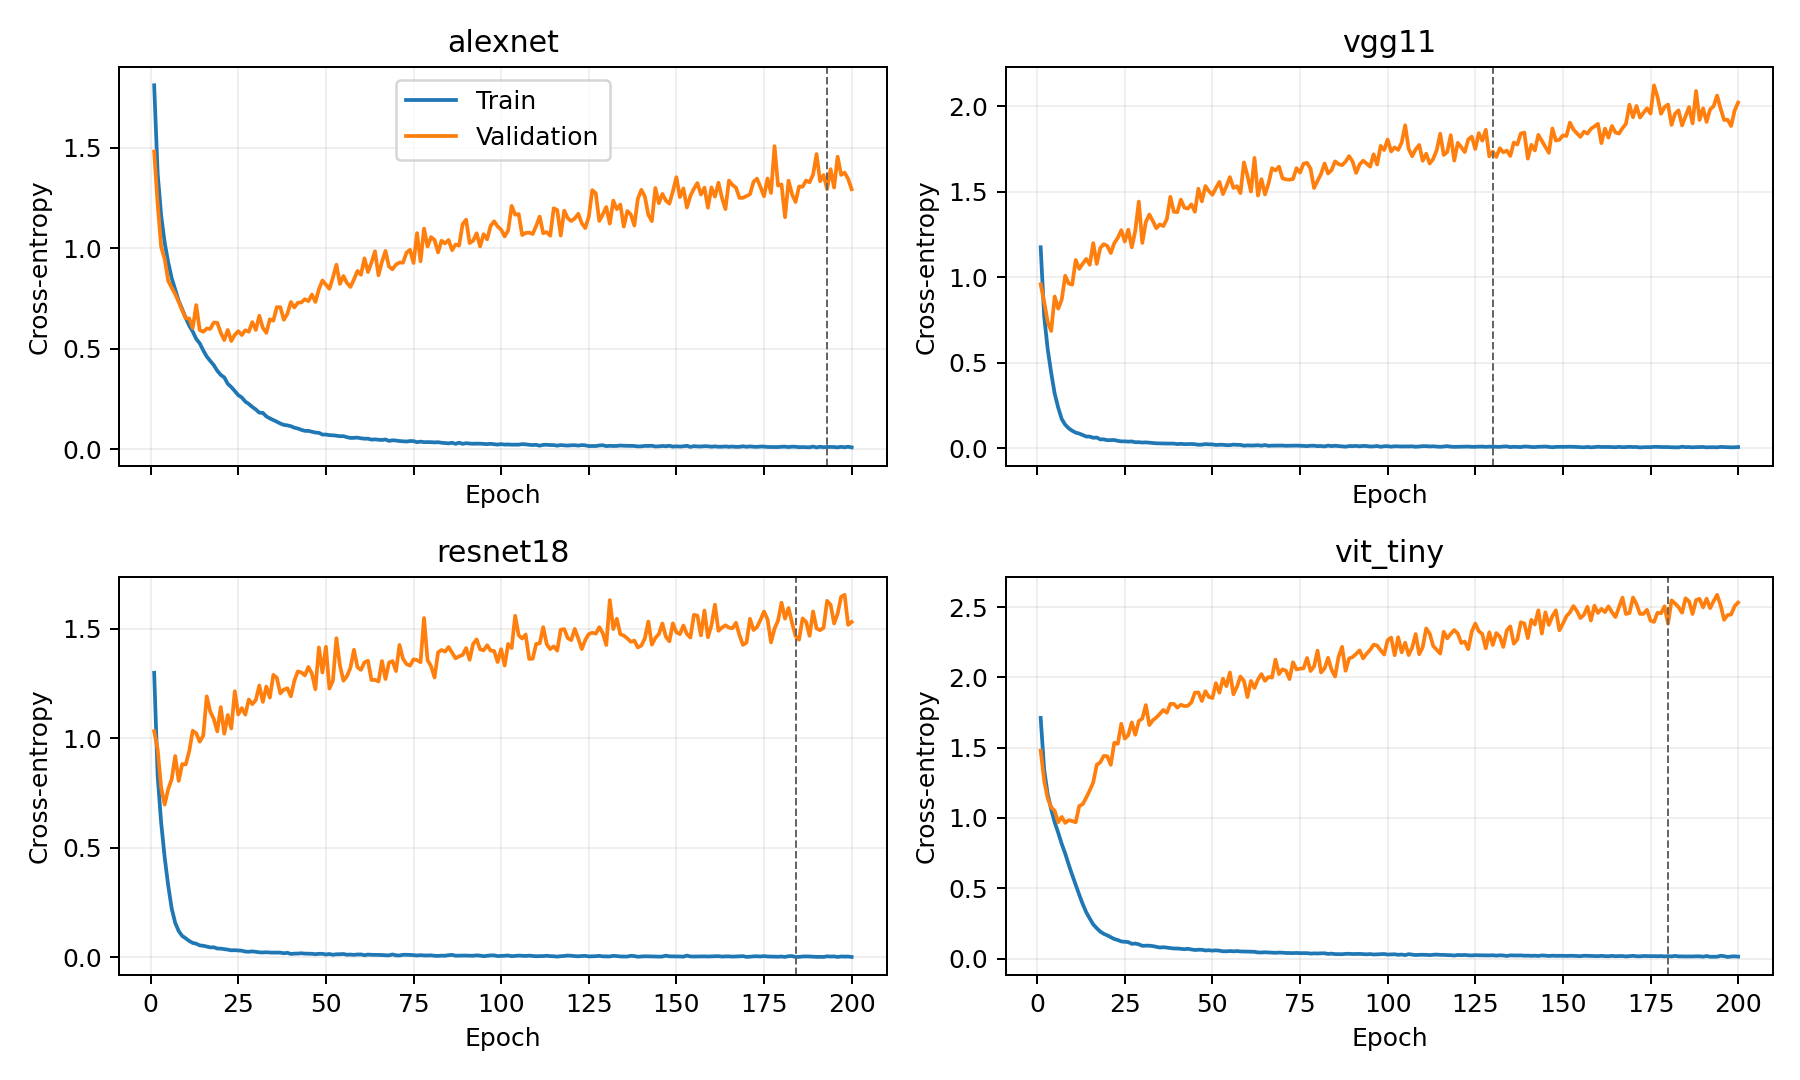
\includegraphics[width=0.90\linewidth]{assets/figures/deep_learning_curves.png}
\caption{Cross-entropy train và validation của bốn mạng; đường dọc đánh dấu epoch có accuracy validation tốt nhất.}
\label{fig:deep-curves}
\end{figure}

Hình~\ref{fig:deep-curves} được dựng trực tiếp từ lịch sử 200 epoch trong
metrics. Loss train giảm xuống rất thấp, trong khi loss validation tăng về
cuối quá trình ở nhiều mạng. Chênh lệch này cho thấy dấu hiệu overfitting;
accuracy validation và cross-entropy không nhất thiết biến thiên cùng chiều.
Vì vậy, việc chọn checkpoint theo validation thay vì dùng epoch cuối là cần thiết.
Các epoch được chọn lần lượt là 193, 130, 184 và 180 cho AlexNet, VGG11-BN,
ResNet18 và ViT tiny.

Bảng~\ref{tab:deep-training} cho thấy VGG11-BN mất khoảng 2,19 giờ huấn luyện,
AlexNet 3,48 giờ, ViT tiny 5,18 giờ và ResNet18 6,51 giờ. Trong lần chạy này,
VGG11-BN có thời gian ngắn nhất, còn AlexNet cho accuracy cao nhất.
Đây là thời gian được ghi bởi chương trình trong quá trình train, bao gồm
đánh giá validation và lưu checkpoint, không phải benchmark suy luận độc lập.
Chi phí còn phụ thuộc thiết bị và cài đặt; 200 epoch giữa các kiến trúc không
đồng nghĩa với cùng lượng tính toán.

\subsection{Phân tích lỗi của mô hình tốt nhất}
\begin{figure}[H]
\centering
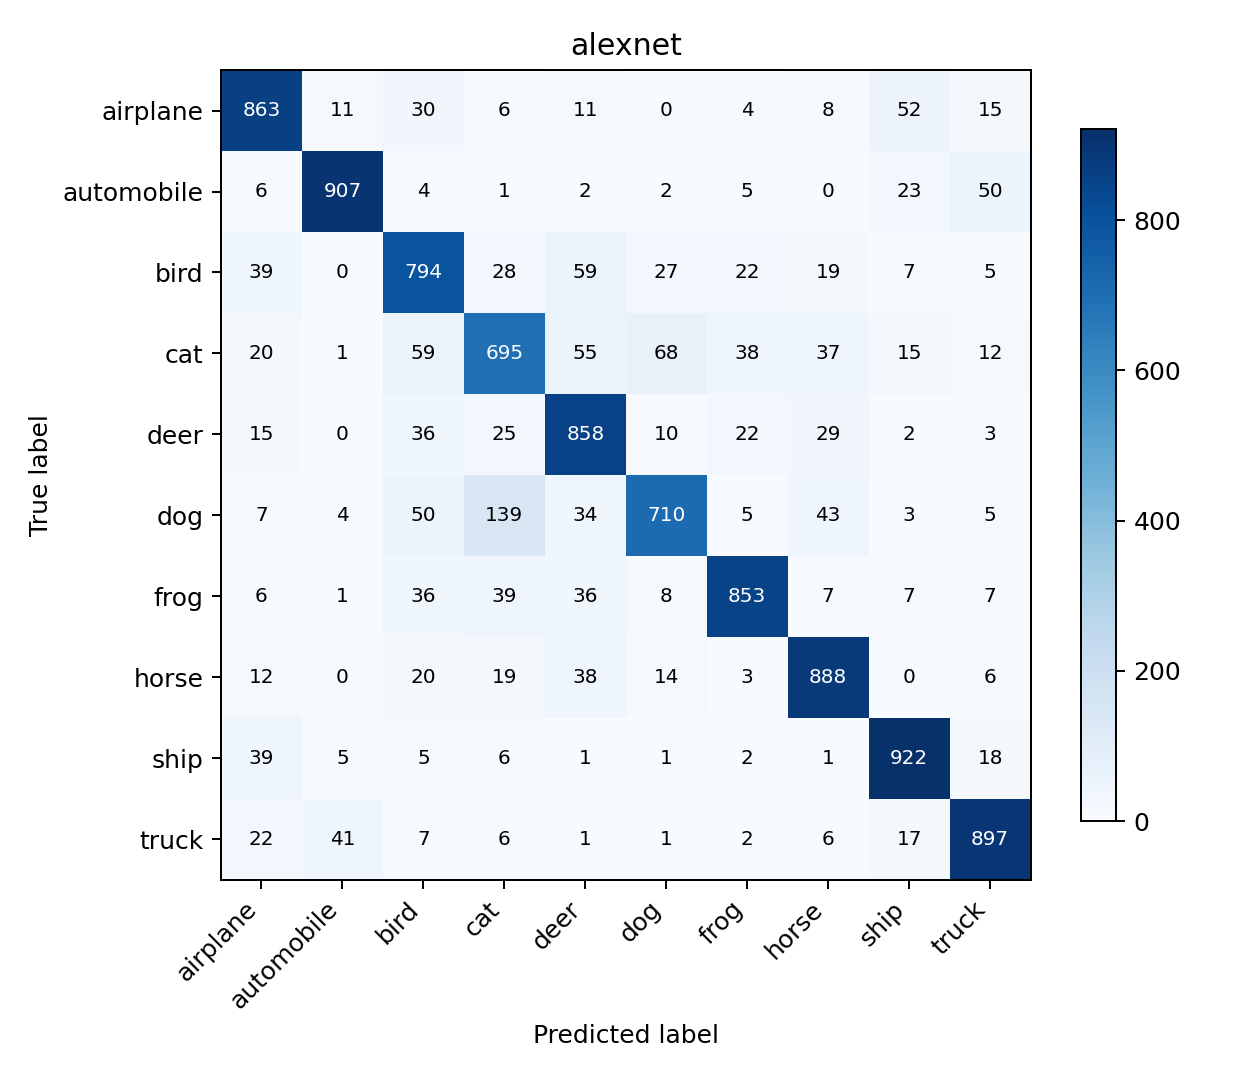
\includegraphics[width=0.65\linewidth]{assets/figures/deep_best_confusion.png}
\caption{Ma trận nhầm lẫn của checkpoint AlexNet được chọn theo validation; hàng là nhãn thật, cột là nhãn dự đoán, mỗi lớp có 1.000 ảnh test.}
\label{fig:deep-confusion}
\end{figure}

Các giá trị trong Hình~\ref{fig:deep-confusion} lấy từ kết quả test đã lưu.
AlexNet đạt F1 cao nhất ở \emph{automobile} (0,9208) và \emph{ship} (0,9004),
trong khi \emph{cat} có F1 thấp nhất (0,7077) và recall 0,695.
Cặp nhầm lẫn lớn nhất là \emph{dog}$\rightarrow$\emph{cat} với 139 ảnh;
chiều ngược lại có 68 ảnh. Hai cặp \emph{bird}$\rightarrow$\emph{deer} và
\emph{cat}$\rightarrow$\emph{bird} đều có 59 ảnh.
Như vậy, học sâu cải thiện kết quả tổng thể nhưng vẫn gặp khó khăn ở một số
lớp động vật. Hình dáng gần nhau ở độ phân giải thấp là một cách giải thích
cần được kiểm tra thêm bằng các ảnh dự đoán sai.

\subsection{Minh họa dự đoán đúng và sai}
Mỗi mô hình được minh họa bằng một ảnh dự đoán đúng (trái, viền xanh) và
một ảnh dự đoán sai (phải, viền đỏ) từ tập kiểm tra. Trong mỗi nhóm đúng
hoặc sai, ảnh được sắp theo cross-entropy và chọn mẫu ở giữa để minh họa.
Điểm softmax trên hình thuộc lớp dự đoán; điểm cao vẫn có thể đi kèm nhãn
sai. Các ảnh này bổ sung góc nhìn trực quan cho kết quả tổng hợp trong
Bảng~\ref{tab:results}.

\begin{figure}[H]
\centering
\begin{minipage}[t]{0.48\linewidth}
\centering
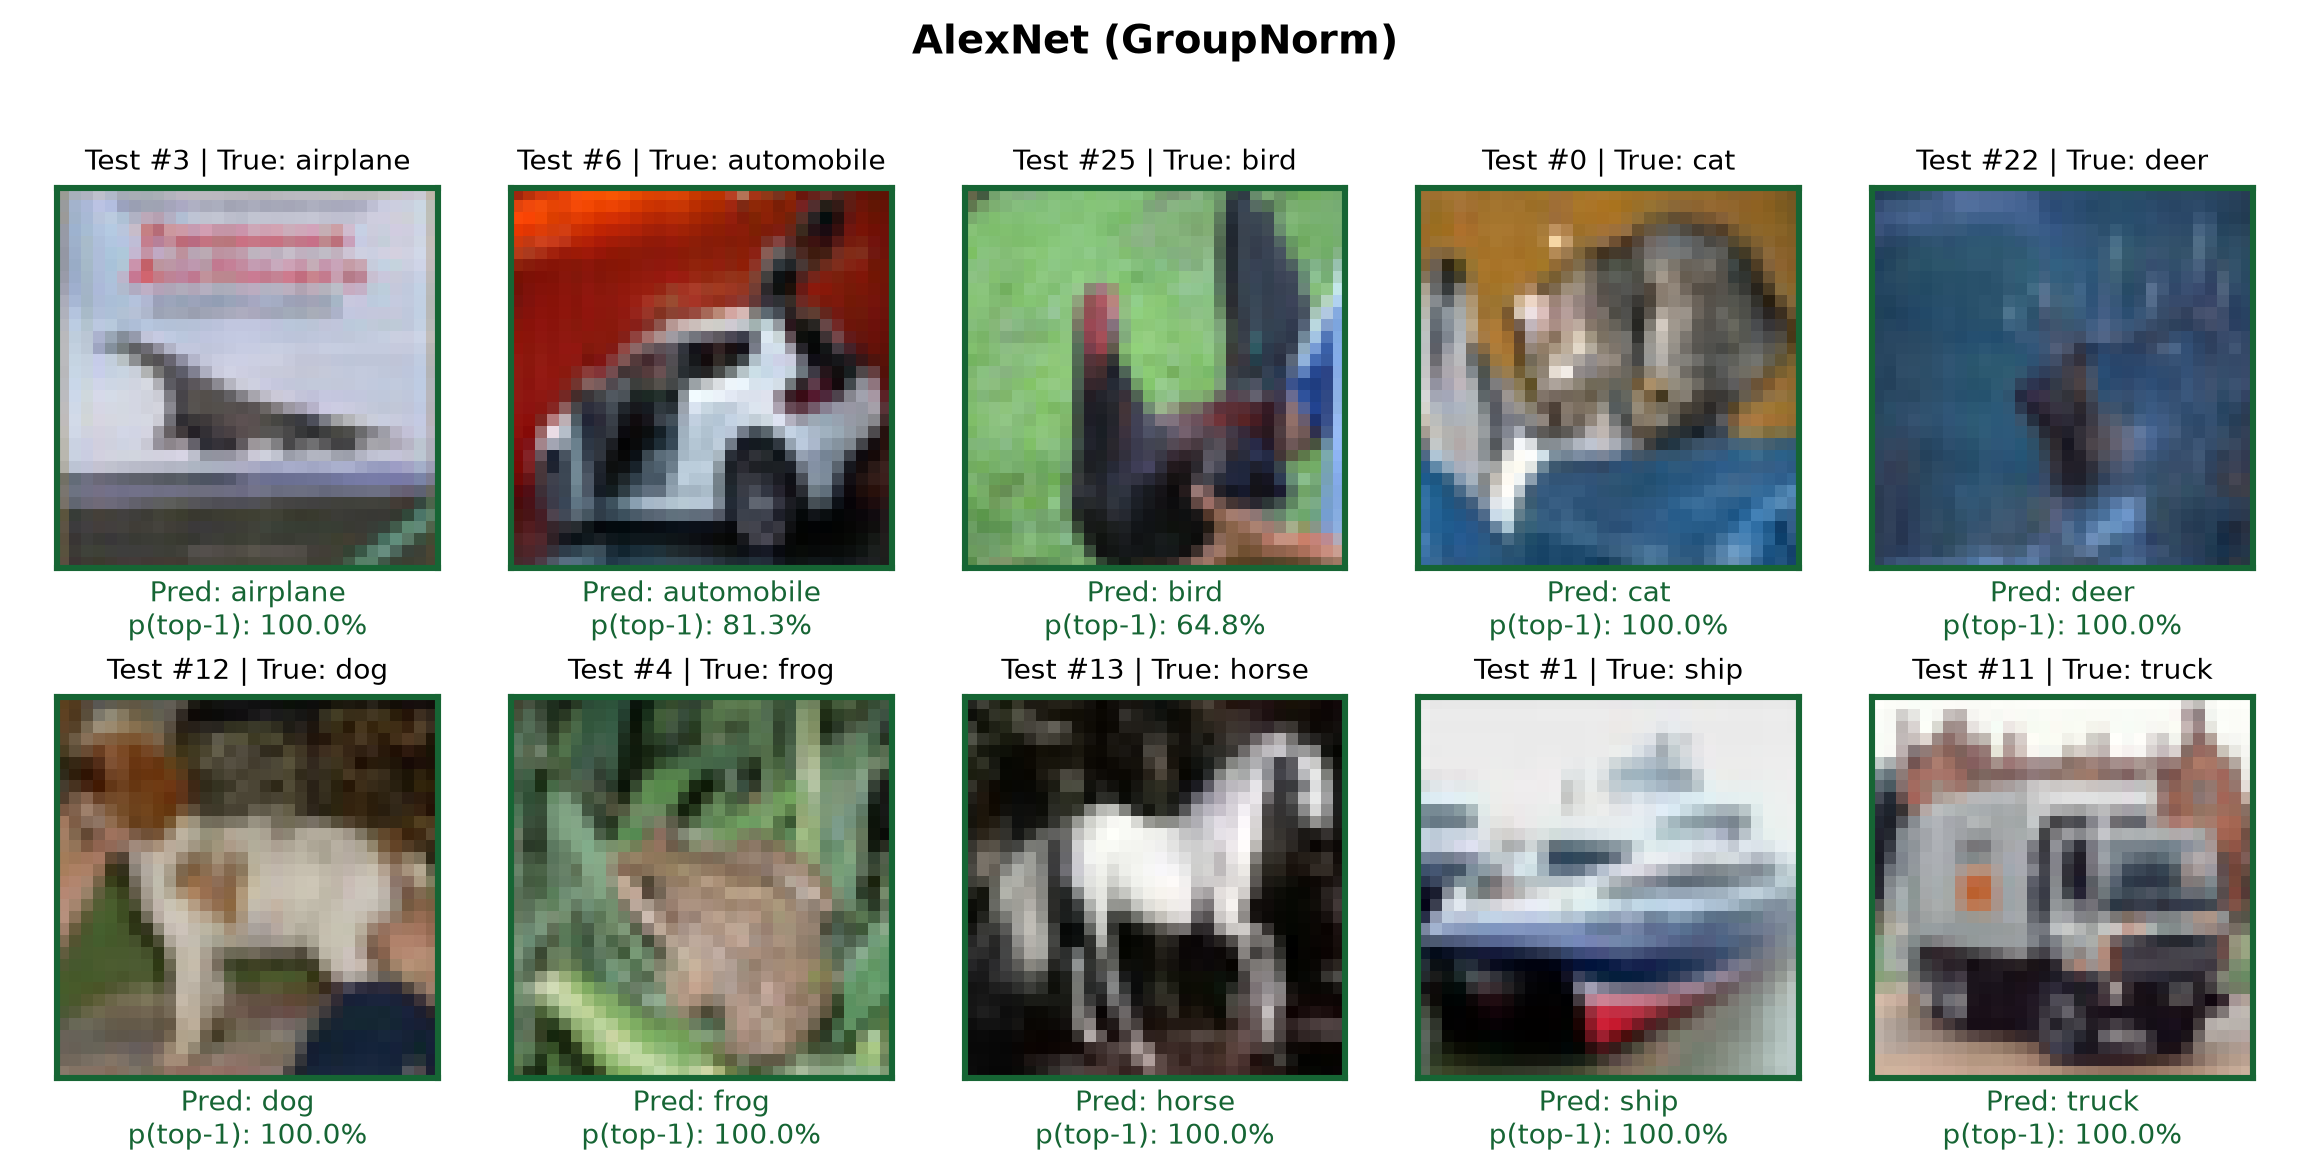
\includegraphics[width=\linewidth]{assets/figures/alexnet_predictions.png}
\caption{Dự đoán của AlexNet ở epoch 193.}
\label{fig:pred-alexnet}
\end{minipage}\hfill
\begin{minipage}[t]{0.48\linewidth}
\centering
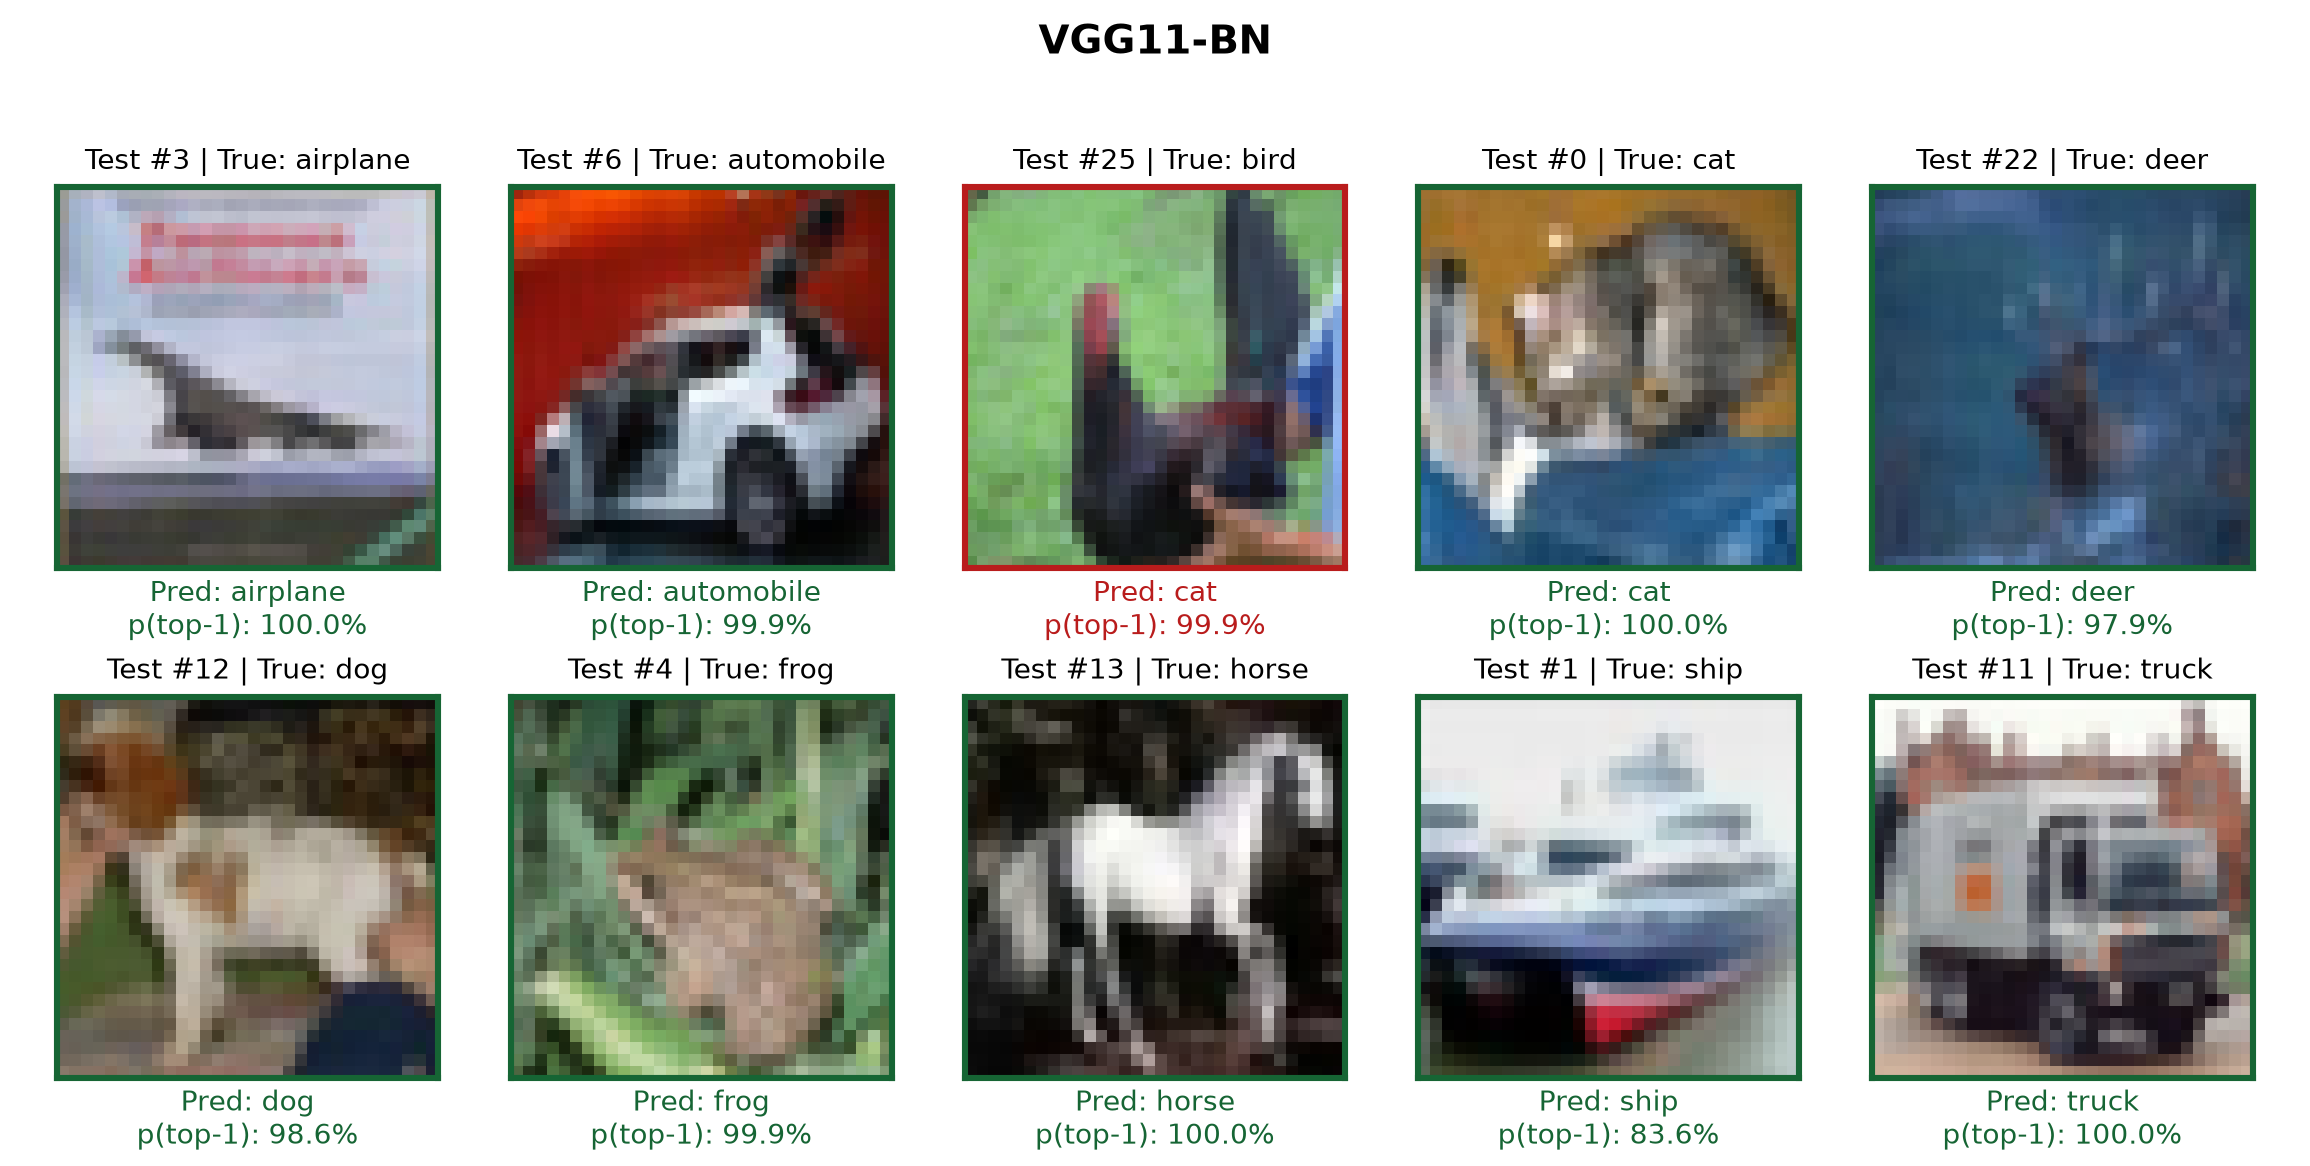
\includegraphics[width=\linewidth]{assets/figures/vgg11_predictions.png}
\caption{Dự đoán của VGG11-BN ở epoch 130.}
\label{fig:pred-vgg}
\end{minipage}
\end{figure}

\begin{figure}[H]
\centering
\begin{minipage}[t]{0.48\linewidth}
\centering
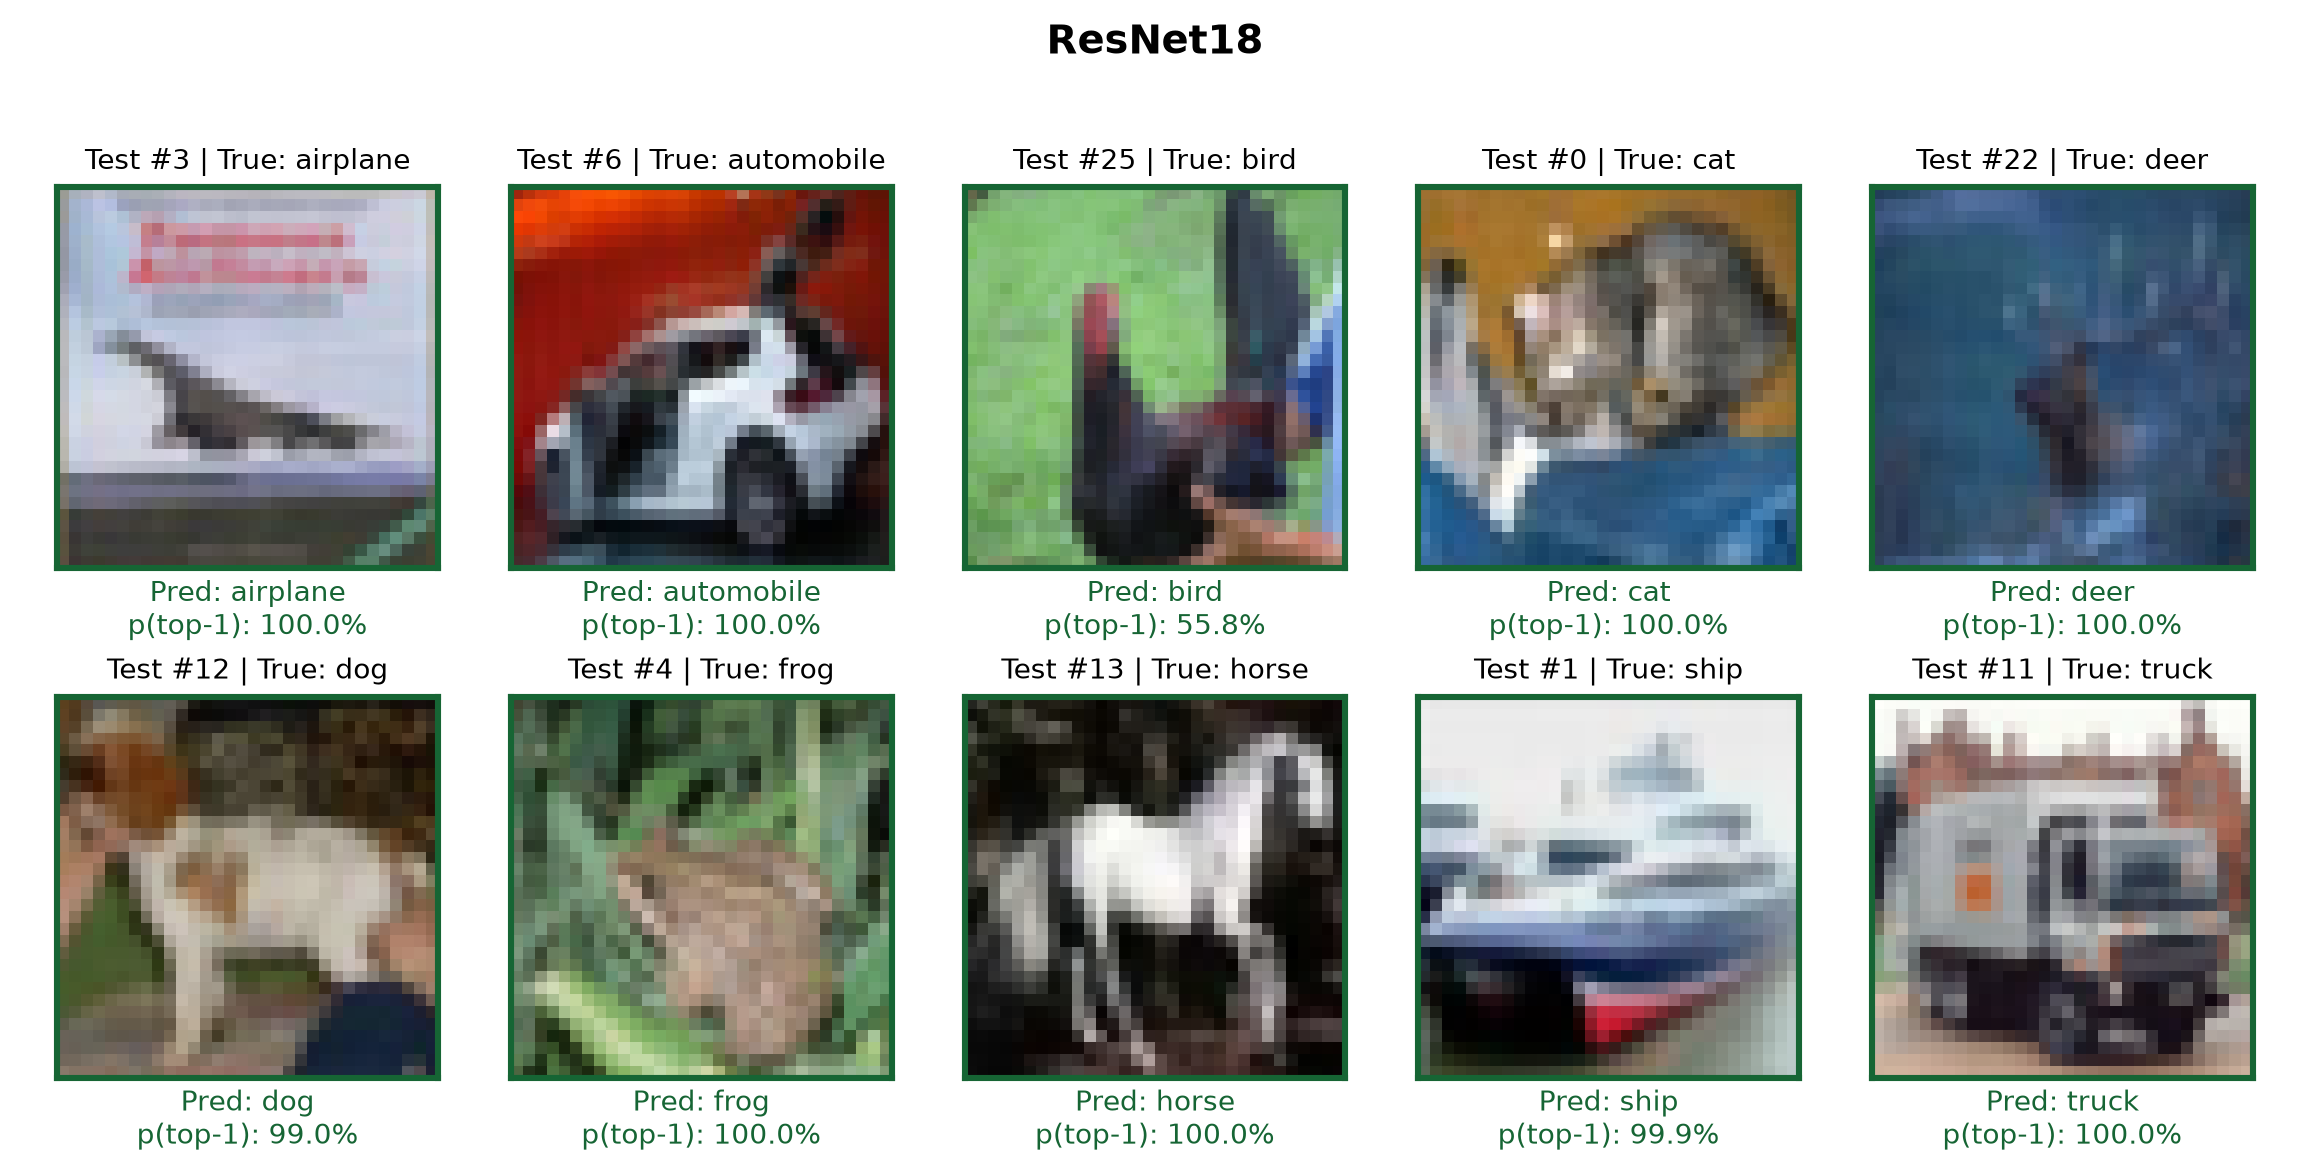
\includegraphics[width=\linewidth]{assets/figures/resnet18_predictions.png}
\caption{Dự đoán của ResNet18 ở epoch 184.}
\label{fig:pred-resnet}
\end{minipage}\hfill
\begin{minipage}[t]{0.48\linewidth}
\centering
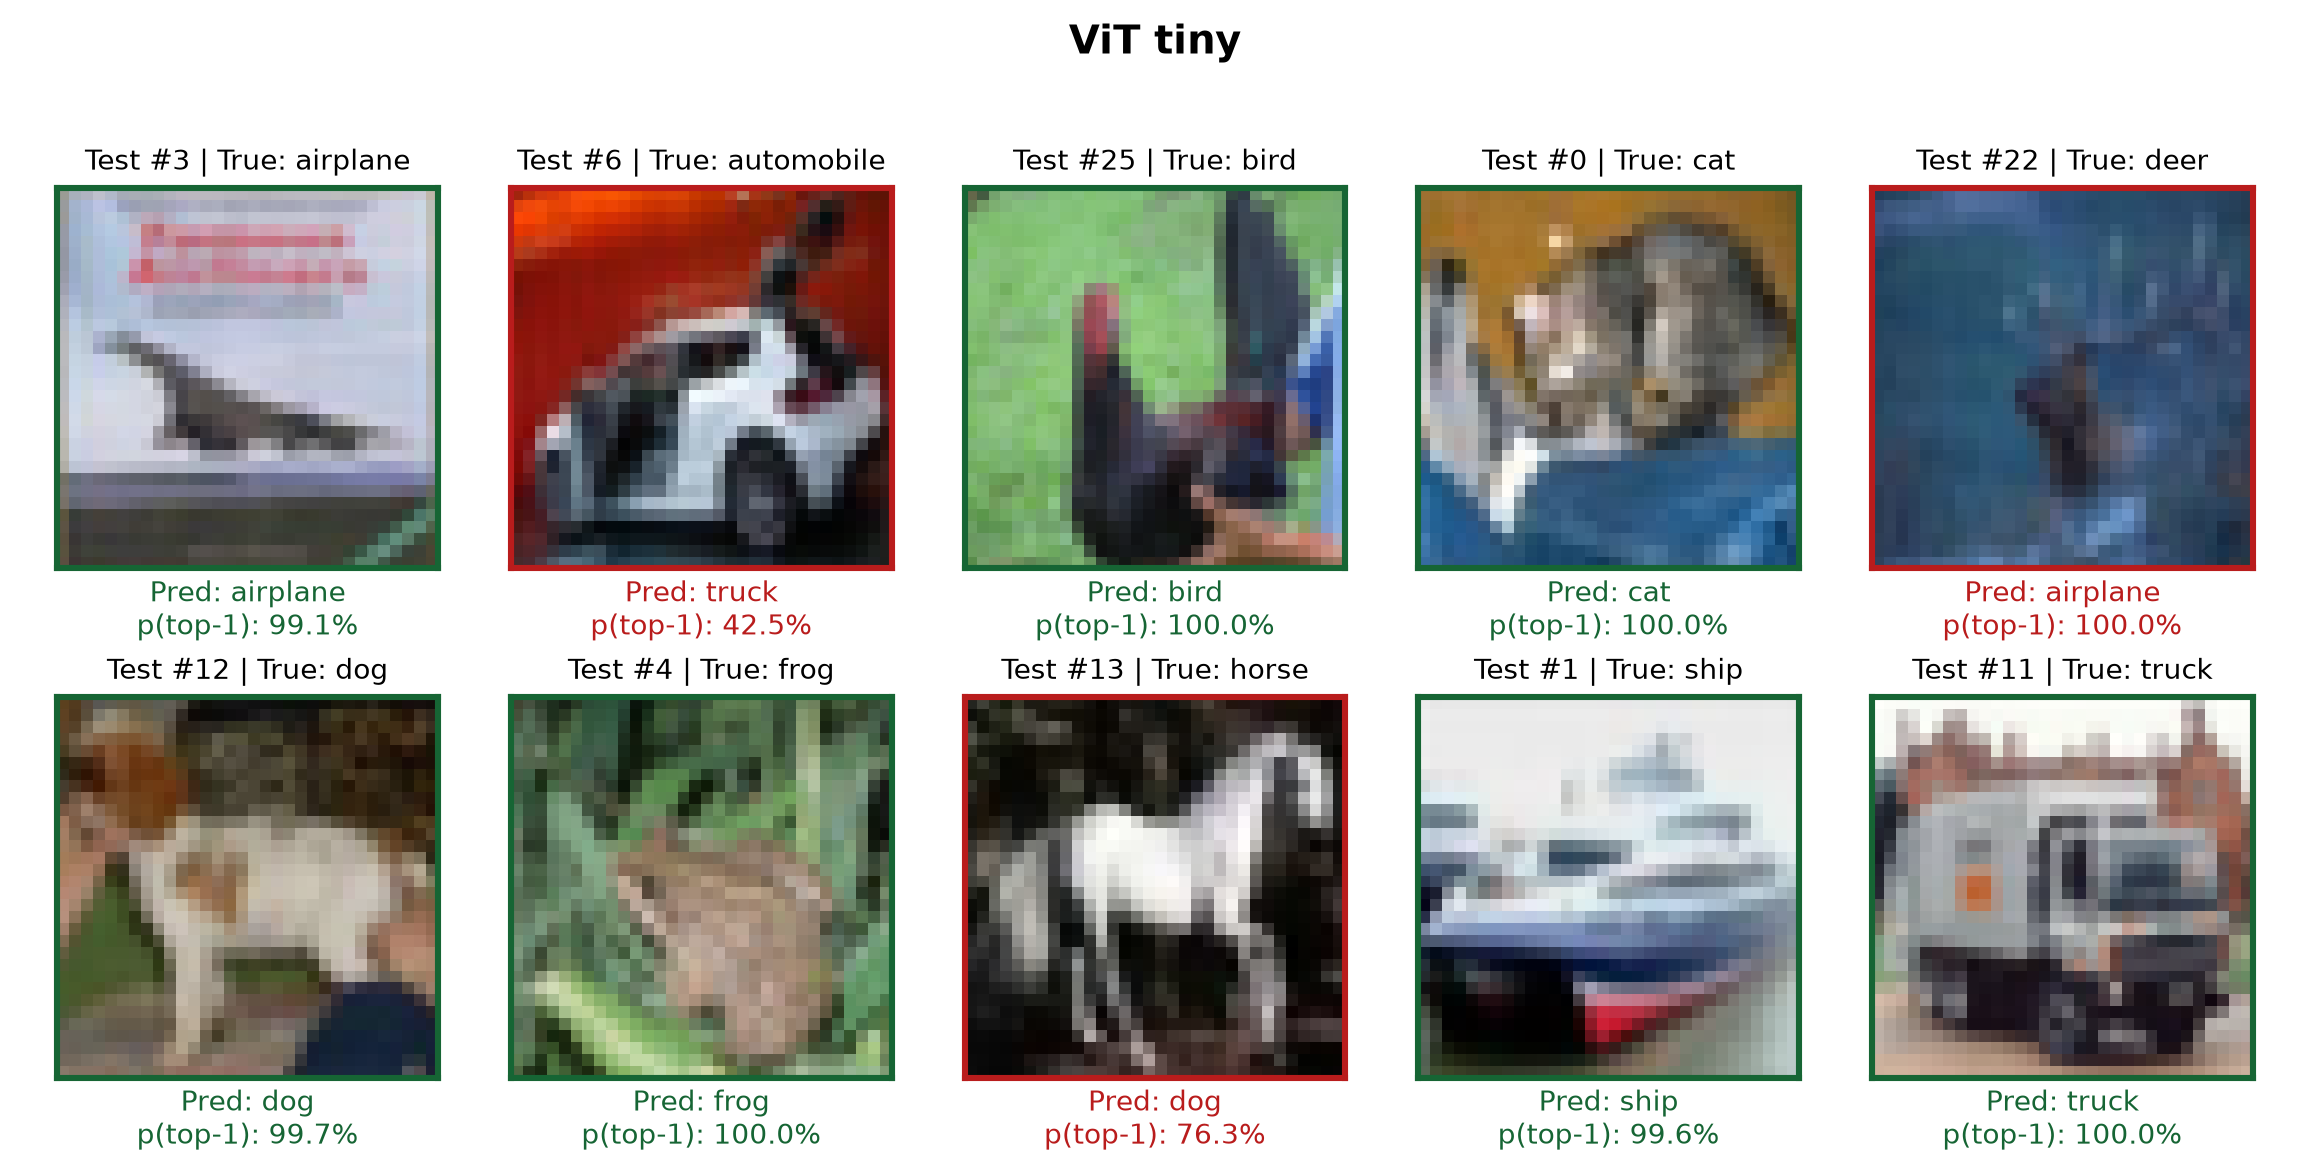
\includegraphics[width=\linewidth]{assets/figures/vit_tiny_predictions.png}
\caption{Dự đoán của ViT tiny ở epoch 180.}
\label{fig:pred-vit}
\end{minipage}
\end{figure}


\section{Kết luận}
Báo cáo đã cài đặt và đánh giá các biến thể AlexNet, VGG11-BN, ResNet18 và
ViT tiny trên CIFAR-10, đồng thời giữ kết quả Pixel, HOG và SIFT phẳng kết hợp
SVM hoặc Random Forest để so sánh. Trên 10.000 ảnh test chính thức, AlexNet đạt
83,87\% accuracy và macro-F1 0,8381, vượt baseline tốt nhất HOG--SVM 30,68 điểm
phần trăm accuracy. ResNet18, VGG11-BN và ViT tiny cũng cao hơn toàn bộ baseline
trong bảng.

Kết quả cho thấy lợi ích của học biểu diễn trực tiếp từ ảnh trong cấu hình
đã khảo sát. CNN đạt kết quả tốt hơn ViT tiny khi cùng huấn luyện từ đầu,
không dùng tăng cường dữ liệu; tuy nhiên một seed và một bộ siêu tham số chưa
đủ để xếp hạng tổng quát các kiến trúc. Hướng cải thiện tiếp theo là tăng cường
dữ liệu, điều chỉnh lịch learning rate và điều chuẩn bằng validation, sau đó
lặp lại với nhiều seed. Tập test cần tiếp tục được giữ cho đánh giá cuối.

\clearpage
\bibliographystyle{plain}
\bibliography{references}
\end{document}
